\documentclass{exam}
\usepackage[utf8]{inputenc}
\usepackage[romanian]{babel}
%\usepackage{lastpage}
\usepackage{enumitem}
\usepackage{listings}
\usepackage{amsmath}
\usepackage{color}
%\usepackage{graphicx}
\usepackage{minted}
% \usepackage{algorithm}
% \usepackage[noend]{algpseudocode}
\usepackage{pxfonts}
%\usepackage{mathtools}
%\usepackage{caption}
\usepackage[linesnumbered,ruled,vlined]{algorithm2e}
% \usepackage{amsmath}
\usepackage[skins]{tcolorbox}

% \pagestyle{headandfoot}
\footer{}{\thepage}{}

\usepackage{hyperref}
\usepackage{url}

% \renewcommand*{\ttdefault}{lmtt}
% \NoCaptionOfAlgo
\SetAlgoCaptionLayout{centerline}
\RestyleAlgo{boxed}
\LinesNotNumbered
% \renewcommand{\fnum@algocf}{Argoritm}%
\SetAlgorithmName{Algoritm}{}{}

% \newcommand{\Read}{\textbf{citește }}
% \newcommand{\And}{\textbf{\emph{și }}}
\newcommand{\code}{\texttt}

\SetKw{Read}{citește}
\SetKwFor{While}{cât timp}{execută}{sfârșit cât timp}
\SetKwFor{For}{pentru}{execută}{sfârșit pentru}
\SetKwIF{If}{ElseIf}{Else}{dacă}{atunci}{altfel dacă}{altfel}{sfârșit dacă}
\SetKw{Write}{scrie}

% \DeclareCaptionFormat{myformat}{#3}
% \captionsetup[algorithm]{format=myformat}
% \captionsetup{labelformat=empty}

% \renewcommand{\algorithmicwhile}{\textbf{cât timp}}
% \renewcommand{\algorithmicdo}{\textbf{execută}}

\definecolor{Brown}{cmyk}{0,0.81,1,0.60}
\definecolor{OliveGreen}{cmyk}{0.64,0,0.95,0.40}
\definecolor{CadetBlue}{cmyk}{0.62,0.57,0.23,0}
\definecolor{lightlightgray}{gray}{0.9}

\lstset{
% language=C++,                             % Code langugage
basicstyle=\ttfamily,                   % Code font, Examples: \footnotesize, \ttfamily
keywordstyle=\bfseries,        % Keywords font ('*' = uppercase)
commentstyle=\color{gray},              % Comments font
columns=flexible,
% numbers=left,                           % Line nums position
% numberstyle=\tiny,                      % Line-numbers fonts
% stepnumber=1,                           % Step between two line-numbers
% numbersep=5pt,                          % How far are line-numbers from code
% backgroundcolor=\color{lightlightgray}, % Choose background color
% frame=none,                             % A frame around the code
% tabsize=2,                              % Default tab size
% captionpos=b,                           % Caption-position = bottom
% breaklines=true,                        % Automatic line breaking?
% breakatwhitespace=false,                % Automatic breaks only at whitespace?
% showspaces=false,                       % Dont make spaces visible
% showtabs=true,                         % Dont make tabls visible
}


\title{Concursul MateInfoUB 2025, secțiunea Informatică}
\vspace{-25mm}
\date{10 Mai 2025}

\begin{document}

\maketitle

Concursul constă în obținerea unui punctaj cât mai mare prin rezolvarea celor 20 de probleme propuse. Fiecare problemă are un punctaj corespunzător gradului ei de dificultate. Cel mai probabil, nu veți avea suficient timp să rezolvați toate problemele. Fiecare problemă are un singur răspuns corect.

\section{Probleme de dificultate scăzută}

%\begin{questions}

%\question 

\subsection*{Problema 1}

(2 puncte) Mara are un seif care se deschide cu un cod PIN  pe care ea l-a uitat. Ea știe că PIN-ul conține exact 5 cifre (de la 0 la 9), iar după introducerea lor trebuie apăsată tasta 0 pentru confirmare. Ca să-și dea seama de cod, Mara examinează cu atenție seiful și observă amprente numai pe butoanele 0, 2, 5 și 8. Întrucât doar ea a folosit seiful și nu a greșit niciodată codul, deduce că ar putea calcula rapid numărul maxim de combinații pe care să le încerce pentru a deschide seiful. Care este acest număr? \\



\begin{oneparchoices}
 \choice 243
 \choice 1024
 \choice 390 (corect)
 \choice 150 
 \choice 240
\end{oneparchoices}
\subsection*{Problema 2}

(2 puncte) Ștefan și-a cumpărat un telefon de ultimă generație, protejat cu un pattern-lock pe o grilă $3 \times 3$. Pentru a debloca aparatul, el trebuie să deseneze cu degetul un pattern care îndeplinește simultan următoarele condiții:

\begin{itemize}
 \item pattern-ul poate porni din orice punct al grilei; 
 \item pattern-ul urmează numai segmente directe între puncte adiacente pe orizontală, verticală sau diagonală (punctele din colțul grilei au trei puncte adiacente, punctul din centru grilei are opt puncte adiacente, iar restul punctelor din grilă au cinci puncte adiacente);
 \item un segment poate fi parcurs cel mult o dată;
 \item pattern-ul se încheie în același punct din care a pornit;
 \item degetul nu se ridică de pe ecran pe tot parcursul desenului.
\end{itemize}

Câte dintre următoarele 6 exemple de pattern-uri respectă regulile date?

\begin{figure}[H]
\centering
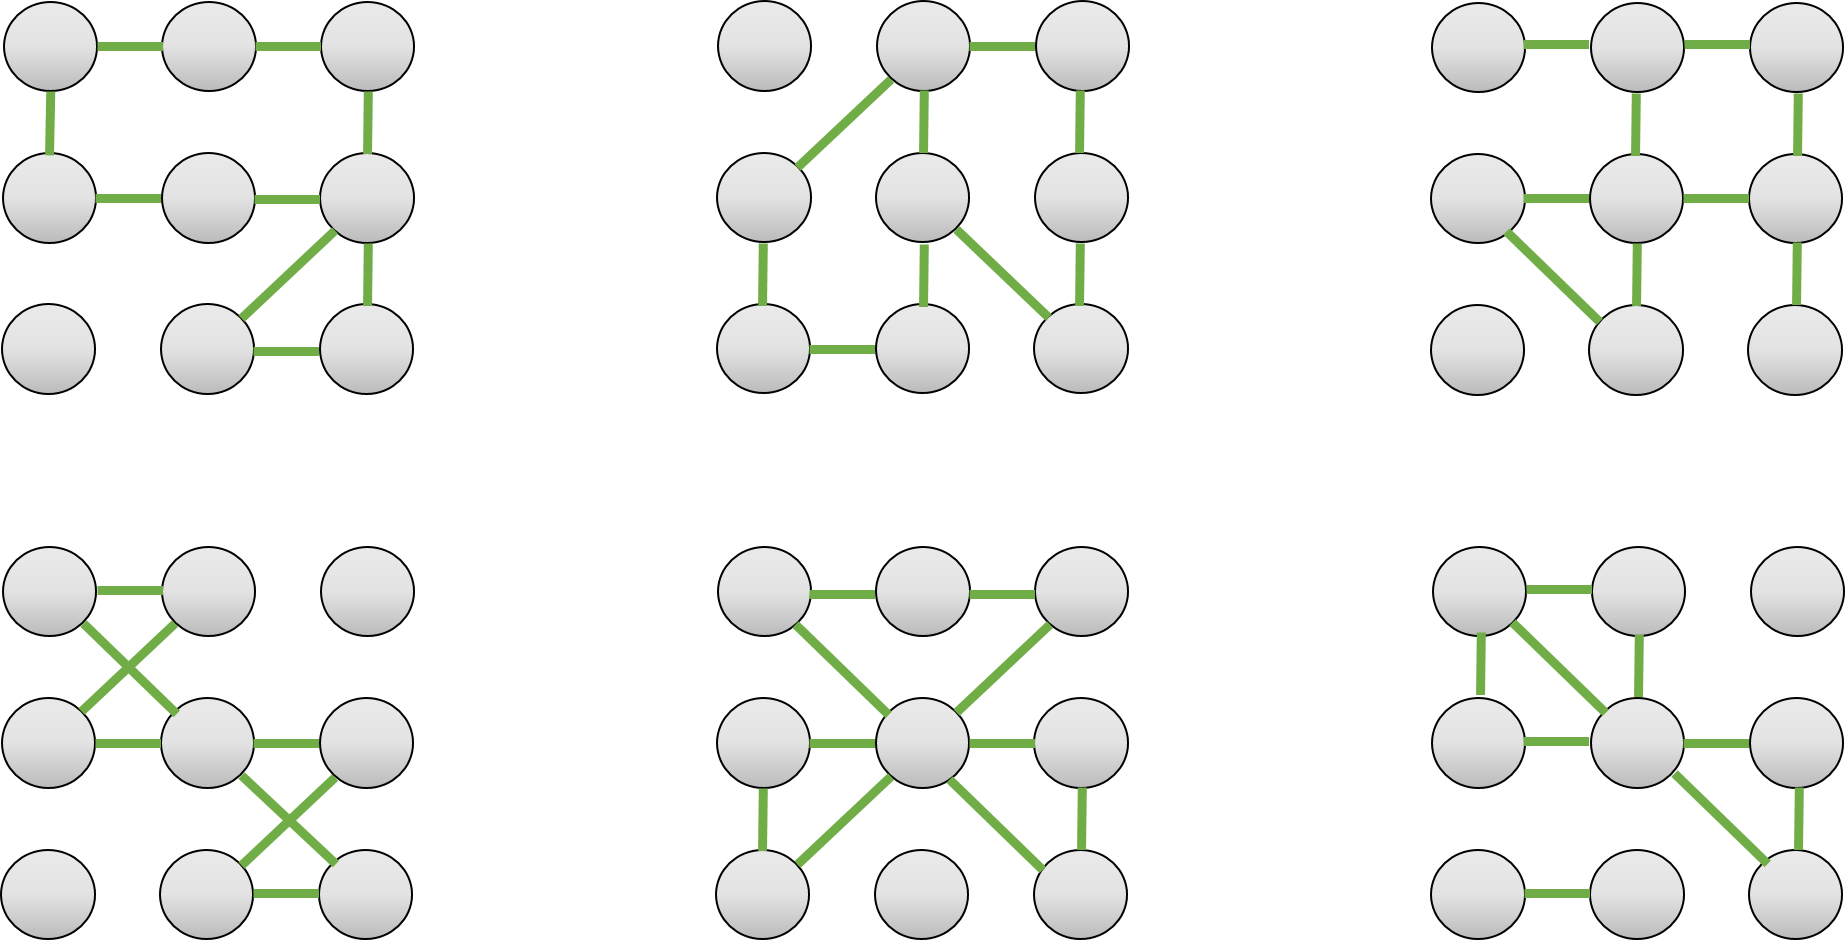
\includegraphics[scale=0.25]{problema2.png}
\end{figure}
\begin{oneparchoices}
 \choice 1
 \choice 2
 \choice 3 (corect)
 \choice 4 
 \choice 5
\end{oneparchoices}
\subsection*{Problema 3}

(2 puncte) Mara a învățat la TIC despre clipboard și despre câteva scurtături utile și dorește să împărtășească tuturor noile ei cunoștințe :
\begin{itemize}
  \item \textbf{Clipboard} - zonă temporară de memorie utilizată de sistemul de operare pentru a stoca date copiate  încât acestea să poată fi lipite (pasted) ulterior într-un alt loc;
  \item \textbf{CTRL+C} – combinație de taste care copiază selecția curentă în clipboard.
  \item \textbf{CTRL+V} – combinație de taste care inserează conținutul copiat din clipboard în poziția curentă a cursorului (clipboard-ul nu se golește). După inserare cursorul se mută la sfârșit, după conținutul inserat.
  \item \textbf{CTRL+A} – combinație de taste care selectează tot conținutul dintr-un document, pagină sau câmp activ. Când \textbf{CTRL+A} este urmat de \textbf{CTRL+C} efectul este următorul: se copiază în clipboard conținutul selectat și cursorul se mută la sfârșit.  Când \textbf{CTRL+A} este urmat de \textbf{CTRL+V} efectul este următorul: se mută cursorul la sfârșit și se copiază în continuare conținutul din clipboard. 
\end{itemize}

Plecând de la textul MIUB2025, Mara folosește o serie de combinații de taste și obține un nou text. Care este lungimea textului rezultat dacă Mara folosește următoarea succesiune: 
$$
\text{CTRL+A} \quad \text{CTRL+C} \quad \text{CTRL+V} \quad \text{CTRL+A} \quad \text{CTRL+V} \quad \text{CTRL+A} \quad \text{CTRL+C} \quad \text{CTRL+V} \quad \text{CTRL+V}
$$
\begin{oneparchoices}
 \choice 40
 \choice 48
 \choice 64
 \choice 72 (corect)
 \choice 96
\end{oneparchoices}

\subsection*{Problema 4}

(2 puncte) Considerăm un joc puzzle în care avem trei litere A, B, C care pot fi puse pe patru poziții (numerotate 1, 2, 3, 4 în figura de mai jos). O configurație inițială conține literele A, B și C puse într-o ordine aleatoare în pozițiile 1, 2 și 3 și poziția 4 din centru goală. Scopul acestui puzzle este ca pornind dintr-o configurația inițială dată să ajungem printr-o serie de mutări (serie eventual vidă) la configurația de referință din figura de mai jos. În această configurație de referință litera A ocupă poziția 1, litera B ocupă poziția 2, litera C ocupă poziția 3, iar poziția 4 rămâne goală.

\begin{figure}[h]
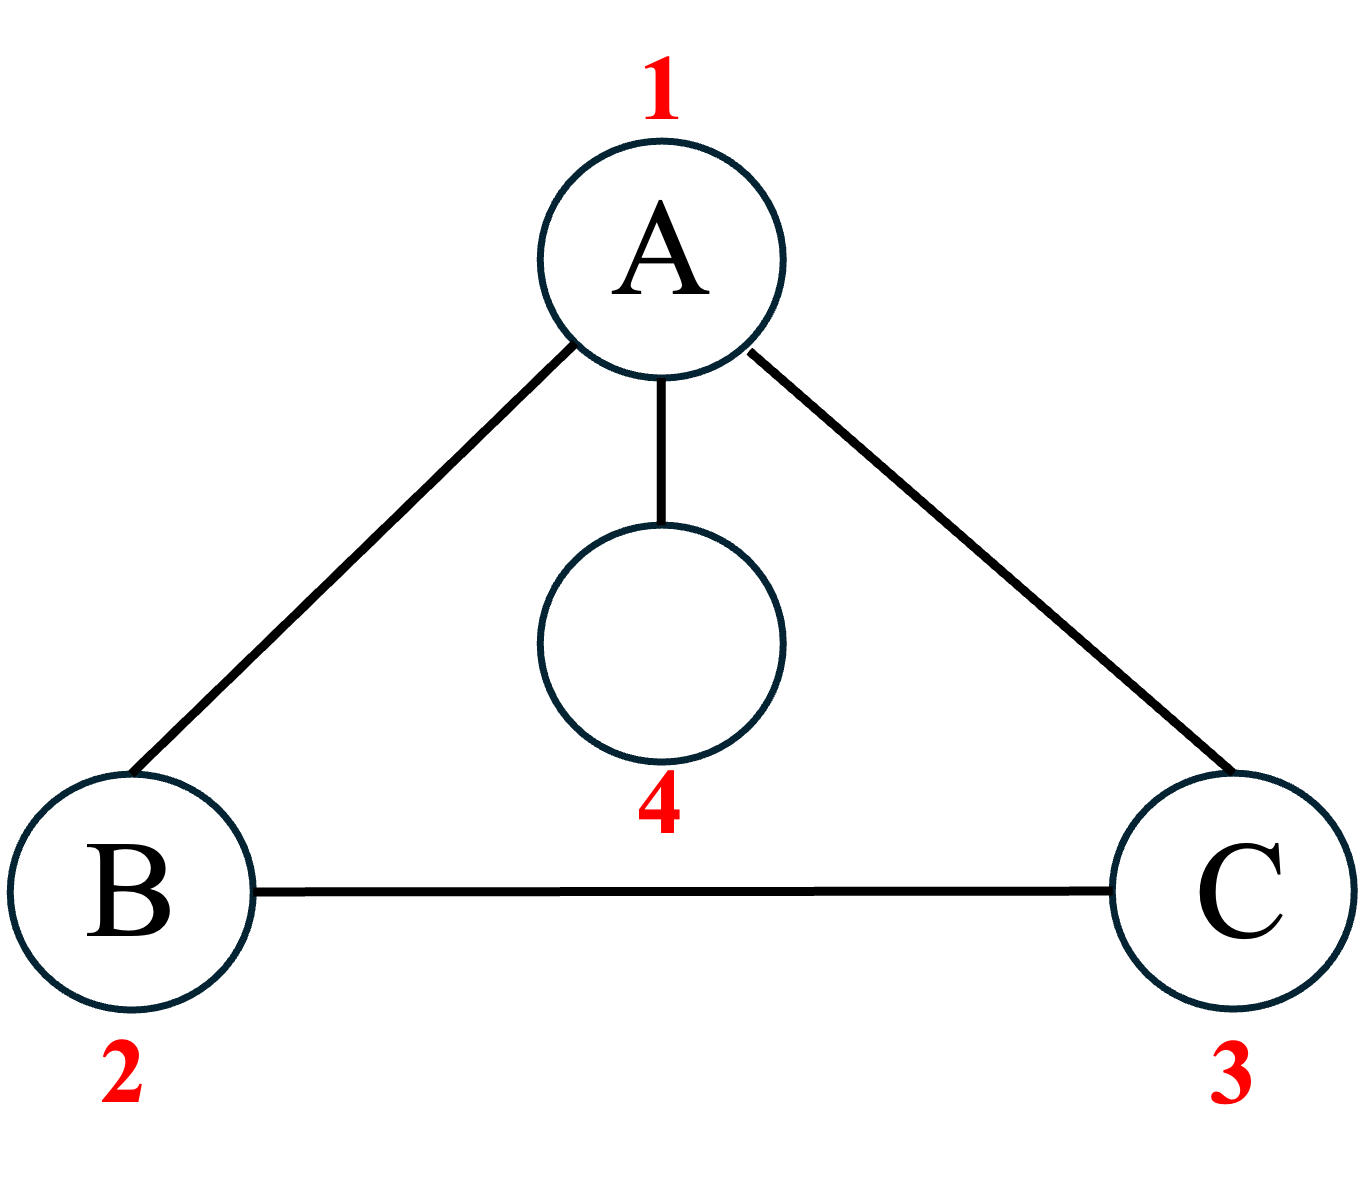
\includegraphics[scale=0.45]{triunghi_ABC_1.png}
\centering
\end{figure}

Putem realiza o mutare deplasând o literă de pe poziția ei curentă în poziția goală, dacă există o linie care conectează cele două poziții. Spre exemplu, pornind din configurația ACB (A pe poziția 1, C pe poziția 2, B pe poziția 3) putem obține configurația de referință prin mutările ilustrate în figura de mai jos.

\begin{figure}[h]
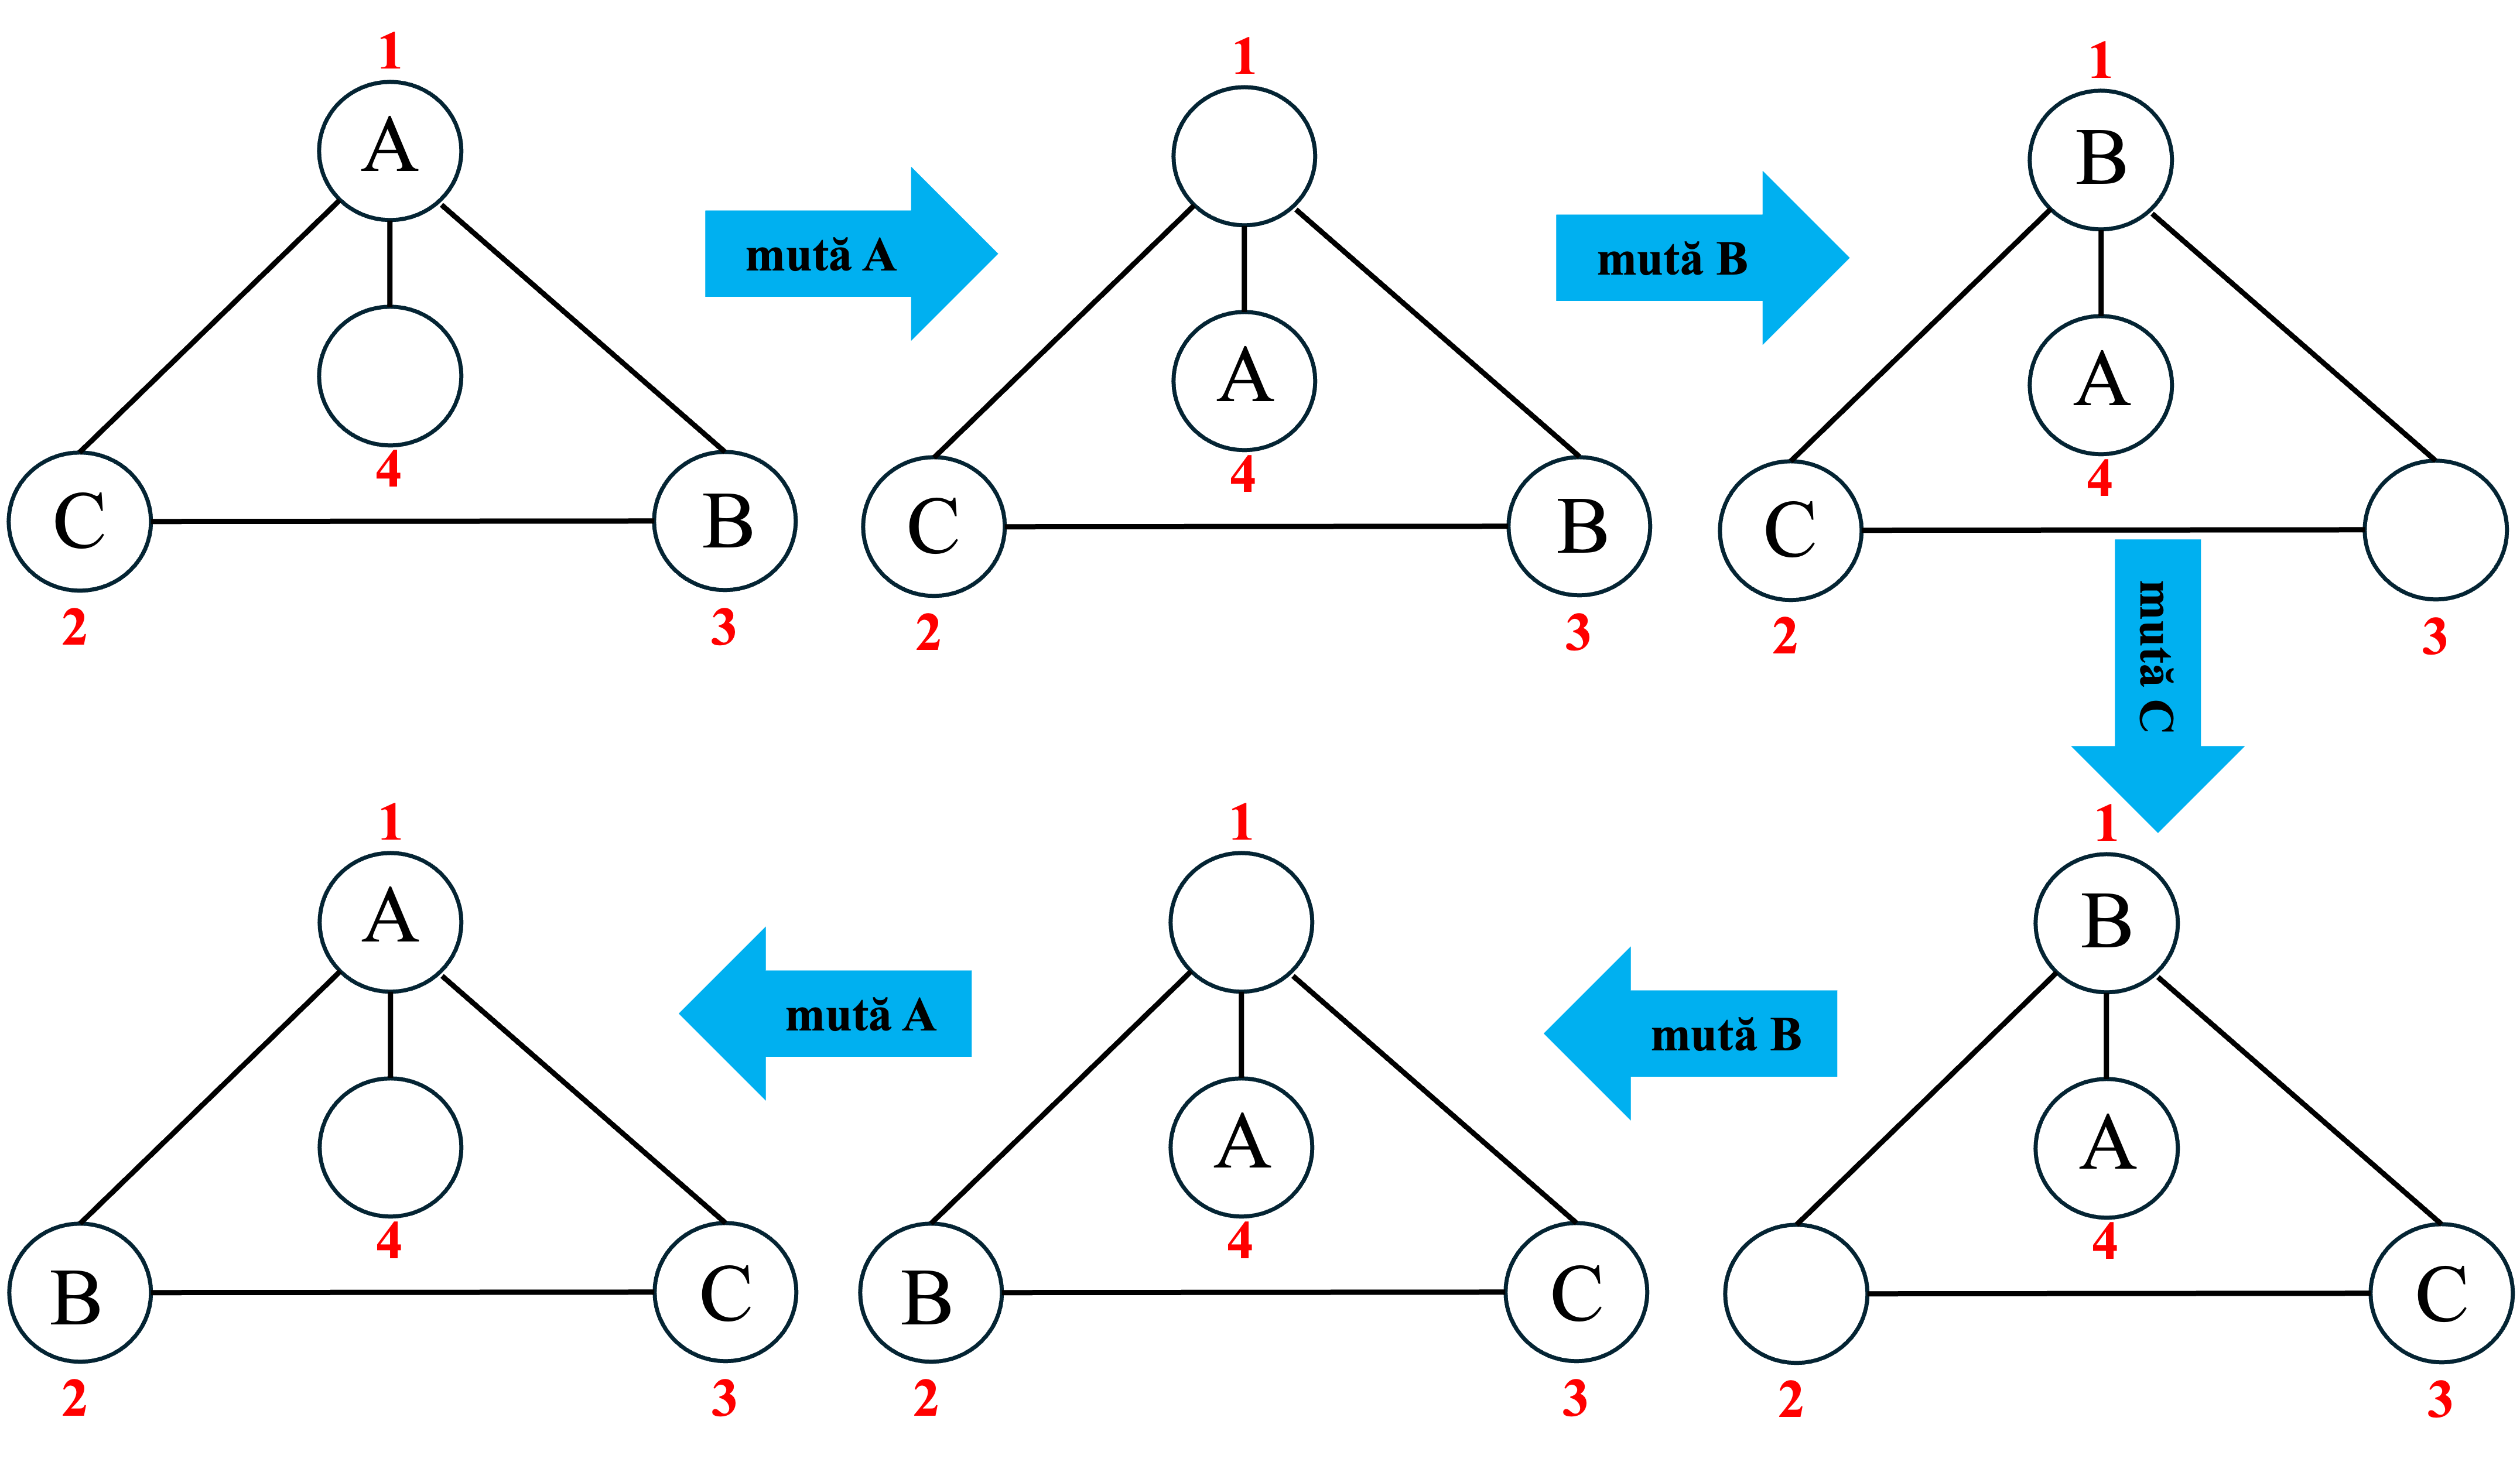
\includegraphics[scale=0.45]{mutare_ABC_config_finala.png}
\centering
\end{figure}

De asemenea, din configurația inițială ABC obținem puzzle-ul dorit fără să fie nevoie să facem vreo mutare. Totuși, nu din orice configurație inițială putem ajunge printr-o serie de mutări la configurația de referință dorită. Considerând toate configurațiile inițiale obținute din permutarea celor trei litere A, B și C din câte aceste configurații nu putem rezolva puzzle-ul?


\begin{oneparchoices}
 \choice 0
 \choice 1
 \choice 2
 \choice 3 
 \choice 4 (corect)
\end{oneparchoices}

\newpage

\subsection*{Problema 5}

(2 puncte)  După doi ani de pauză, Furnicuța vrea din nou să se deplaseze pe o frunză, de data aceasta reprezentată printr-o matrice pătratică, formată din $n^2$ celule. Furnicuța este în colțul din stânga-jos al frunzei și vrea să ajungă în colțul din dreapta-jos al frunzei (evident, fără să iasă de pe frunză). La un pas,
ea poate urca de la colțul stânga-jos al unei celule la colțul dreapta-sus al celulei sau poate coborî din colțul stânga-sus al unei celule la colțul dreapta-jos al celulei.
 De exemplu, în figura de mai jos traseul (a) este valid, dar (b) nu este, deoarece Furnicuța a urcat la un pas din colțul dreapta-jos al unei celule în colțul din stânga-sus. Fie $m$ numărul total de  trasee valide pe care le poate face Furnicuța pe o frunză cu $10 \times 10$  celule. Ce valoare are $ m \mbox{ mod }  100$ (restul impărțirii lui $m$ la $100$)?

\begin{figure}[h]
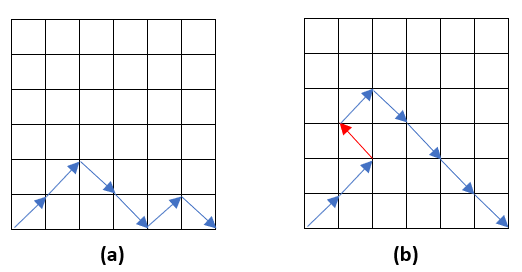
\includegraphics[scale=1]{trasee.png}
\centering
\end{figure}

\begin{oneparchoices}
\choice   24
 \choice   42 (corect)
  \choice  0
 \choice  96
 \choice  76
\end{oneparchoices}

\subsection*{Problema 6}

(2 puncte) Alexandru are un pachet cu 52 de cărți de joc ordonat (de la As la Rege, întâi romb, urmat de treflă, inimă roșie și, în final, inimă neagră).

Alexandru extrage 4 carți consecutive din pachet și primele 3 sunt de inimă roșie. Care este probabilitatea ca și a patra carte să fie tot inimă roșie?

% Sunt 11 moduri de-a scoate 4 carti consecutive, cu primele 3 inima rosie.
% Din ele, 10 sunt bune. Totul este echiprobabil.

\begin{oneparchoices}
 \choice $\frac{10}{11}$ (corect)
 \choice $\frac{13}{25}$
 \choice $\frac{4}{13}$
 \choice $\frac{10}{49}$
 \choice $\frac{1}{13}$
\end{oneparchoices}


\subsection*{Problema 7}

(2 puncte) Scara laterală din Universitatea din București este magică. Conectează cele $N$ etaje, numerotate de la $0$ la $N - 1$, și are următoarea proprietate:

De la etajul $i$, urcând sau coborând pe scară, Matei ajunge magic la etajul $(i+6)\textrm{ (mod N)}$, respectiv $(i - 6)\textrm{ (mod N)}$.
Pentru care din următoarele valori ale lui $N$ poate Matei ajunge de la etajul $0$ la etajul $1$ (urcând și / sau coborând oricât)?  

% N trebuie sa fie prim cu 6 (i.e. sa nu se divida nici cu 2 nici cu 3).

\begin{oneparchoices}
 \choice $2022$
 \choice $2023$ (corect)
 \choice $2024$
 \choice $2025$
 \choice $2026$
\end{oneparchoices}


\subsection*{Problema 8}

(2 puncte) La un concurs de biciclete, concurenții au un traseu format dintr-o urcare urmată de o coborâre. Distanța parcursă la urcare este egală cu distanța parcursă la coborâre (fiecare reprezentând jumătate din lungimea totală a traseului). Unii cicliști urcă mai repede, dar coboară mai încet, și invers. 

%Având în vedere că știți vitezele medii de urcare și coborâre, cine câștigă concursul (adică cine parcurge traseul total în cel mai scurt timp)?

%Cine câștigă concursul avand in vedere ca vitezele concurenților (în km/oră) sunt:

Care dintre concurenții de mai jos, pentru care sunt date vitezele medii de urcare și coborâre (în km/h), va câștiga concursul (adică va parcurge traseul complet în cel mai scurt timp)?

\begin{oneparchoices}
    \choice Bogdan vitezomanul: urcă cu 10, coboară cu 100.
    \choice Vasilică: urcă cu 12, coboară cu 60.
    \choice Emil: urcă cu 20, coboară cu 40.
    \choice Eduard: urcă cu 25, coboară cu 30.  (corect)
    \choice Sorinel fricosul: urcă cu 32 și coboară cu 20.
\end{oneparchoices}


 %\choice{}

\subsection*{Problema 9}

(2 puncte) Alex îi povestește Andreei despre numărul lui preferat.\\
Alex: Numărul meu preferat are 3 cifre, același număr de divizori ca răsturnatul lui și suma cifrelor sale este 20. \\
Andreea: Nu reușesc să ghicesc numărul! \\
Alex: Produsul cifrelor este 288. \\
Andreea: Bine, am găsit numărul! \\

În ce interval se află numarul preferat al lui Alex?


\begin{oneparchoices}
    \choice Între $0$ și $199$.
    \choice Între $200$ și $399$.
    \choice Între $400$ și $599$.
    \choice Între $600$ și $799$ (corect).
    \choice Între $800$ și $999$.
\end{oneparchoices}



\subsection*{Problema 10}

(2 puncte) Meșterul Piperel are $10$ țevi cu lungimile de $7, 5, 3, 2, 3, 10, 7, 4, 9$ și $6$ metri pe care trebuie să le îmbine într-o singură țeavă. De fiecare dată, Piperel poate să îmbine doar două țevi, iar țeava nou obținută va fi așezată lângă celelalte țevi. Îmbinarea a două țevi cu lungimi de $x$ și $y$ metri are un cost egal cu $x + y$ RON și se obține o nouă țeavă cu lungimea $x + y$ metri. Știind că țevile se pot îmbina în orice ordine, calculați costul minim necesar pentru a îmbina toate cele 10 țevi într-una singură.

\begin{oneparchoices}
 \choice 56
 \choice 180 (corect)
 \choice 194
 \choice 278
 \choice 325
\end{oneparchoices}

\section{Probleme de dificultate medie}

\subsection*{Problema 11}

(3 puncte) Cristian și Vlad au un pachet cu 52 de cărți de joc și au inventat un joc cu următoarele reguli:
\begin{itemize}
    \item inițial se aleg N cărți din cele 52 inițiale. Ambii jucători știu valoarea lui N. 
    \item Cristian e primul care ia cărți din pachetul de N cărți, apoi jucătorii alternează.
    \item la fiecare tură jucătorul curent poate lua din pachet exact 2, 3 sau 5 cărți.
    \item dacă la începutul unei ture  numărul de cărți rămase în pachet este 0 sau 1, jucătorul căruia îi este rândul să ia cărți din pachet nu are o opțiune validă și pierde, iar adversarul câștigă.
\end{itemize}


Amândoi jucătorii joacă optimal, evitând orice decizie care i-ar conduce sigur la pierdere dacă există o alternativă câștigătoare. Se desfășoară cinci jocuri, în care se aleg inițial valorile $N = 10$, $N = 20$, $N = 30$, $N = 40$, $N = 50$. Câte dintre aceste jocuri îi revin lui Cristian?

\begin{oneparchoices}
 \choice 1
 \choice 2
 \choice 3
 \choice 4
 \choice 5
\end{oneparchoices}

\subsection*{Problema 12}

(3 puncte) Într-un vis, Mariei i se dezvăluie prețul unui caiet pentru următoarele $10$ zile. În fiecare zi, poate cumpăra un caiet dacă nu are niciunul sau vinde caietul dacă are unul. În mod particular, Maria nu poate deține 2 caiete în același timp, dar poate cumpăra și vinde caiete de oricâte ori dorește.

Prețul unui caiet în următoarele $10$ zile (în lei) este:

$$
15, 31, 5, 15, 20, 5, 17, 23, 10, 18
$$

Care este suma maxima de bani pe care o poate câștiga, știind ca nu deține niciun caiet în prima zi?

% a = [15, 31, 5, 15, 20, 5, 17, 23, 10, 18]
% sum(max(0, i[1] - i[0]) for i in zip(a, a[1:]))


\begin{oneparchoices}
 \choice 26
 \choice 18
 \choice 31
 \choice 57 (corect)
 \choice 72
\end{oneparchoices}

\subsection*{Problema 13}

(3 puncte) Comanda \textit{sensors} din Linux afișează informații despre diferite componente din calculator, inclusiv temperatura. De exemplu:

\begin{minted}{shell}
theodor@lapttop ~> sensors
hygrometer-sensor-2189
Adapter             : ISA interface
signal_strength     : -67 dBm
temperature         : 56 °C
viewing_angle       : 126 °
contrast            : 96 %
brightness          : 61 %

microphone-governor-5104
Adapter             : mSATA adapter
size                : 94 MB
temperature         : 49 °C
load                : 87.18 %
charge_time         : 3 hours
response_time       : 8.55 ms
\end{minted}

% Linkul nu e bun, trebuie sa facem altul.
Matei a rulat comanda și a obținut rezultatul acesta: \url{https://tinyurl.com/mateinfoUB-sensors}.

Câte componente din calculatorul lui au o temperatură strict mai mare decât $80^{\circ}C$?

% lines = open("sensors.txt").readlines()
% lines = [l for l in lines if "°C" in l]
% lines = [l.split(":")[1].split("°C")[0].strip() for l in lines]
% lines = [int(l) for l in lines]
% lines = [l for l in lines if l > 80]
% print(f"Number of devices with temperature above 80 °C: {len(lines)}")


\begin{oneparchoices}
 \choice 345 (corect)
 \choice 346
 \choice 347
 \choice 348
 \choice 349
 \choice 350
 \choice 341
\end{oneparchoices}

\subsection*{Problema 14}

(3 puncte) Ca un om normal, Matei vrea să își conecteze cele $40$ de difuzoare bluetooth la telefon. Telefonul și fiecare din dispozitive se poate conecta simultan la 3 alte dispozitive, și latența fiecărei conexiuni este de exact o milisecundă. Care este latența minimă pe care o poate obține Matei între telefon si cel mai departat difuzor?

% 0 ms: laptopul.
% 1 ms: 3 difuzoare (3 in total)
% 2 ms: 6 difuzoare (9 in total)
% 3 ms: 12 difuzoare (21 in total)
% 4 ms: 19 difuzoare (40 in total)

\begin{oneparchoices}
 \choice 3
 \choice 4 (corect)
 \choice 5
 \choice 6
 \choice 7
 \choice 8
 \choice 9
\end{oneparchoices}



\subsection*{Problema 15}

(3 puncte) Țara Numberland are o sută de mii de orașe, numerotate $1, 2, \dots, 100000$.


Între orașul $i$ și orașul $j$:
\begin{itemize}
    \item Dacă $(i - j)\textrm{ (mod 5)} \leq 2$, atunci există o autostradă directă, de lungime $|i - j|$.
    \item În caz contrar, există o cale ferată directă, de lungime $|i - j|$. 
\end{itemize}

Reamintim că $a\textrm{ (mod $b$)}$ este restul împarțirii lui $a$ la $b$. De exemplu, $-3 \textrm{ (mod 5)} = 2$.

De exemplu, un tren poate ajunge din orașul $1$ în orasul $2$ cu o distanță totală de $7$:
\begin{itemize}
    \item Din orașul $1$ merge în orașul $5$ (distanță $4$).
    \item Din orașul $5$ merge în orașul $2$ (distanță $3$).
\end{itemize}

Distanța dintre două orașe este distanța minimă cu trenul sau cu mașina între cele două orașe. Care este suma distanțelor dintre toate orașele?

% Intre oricare orașe i si j exista drum de distanța |i - j|.
% Asadar, pentru fiecare oras i, avem distanta 1 pana la i+1, 2 pana la i+2 ...
% print(sum(i * (i + 1) // 2 for i in range(100_000)))


\begin{oneparchoices}
 \choice 111113333440000
 \choice 333333333400000
 \choice 333343333400000
 \choice 166671666750000
 \choice 166666666650000 (corect)
 \choice 166666766600000
 \choice 366666766600000
\end{oneparchoices}



\subsection*{Problema 16}

(3 puncte) Are tata două fete. Perfecționist, vrea să se asigure că numele celor două fete să fie la aceeași \textit{distanța de editare} de numele \texttt{elma}, așadar consideră mai multe opțiuni.

Pentru perechile de nume care conțin \texttt{*}, cele două nume sunt la aceeași distanță de \texttt{elma} dacă există \textbf{cel putin} o modalitate de-a înlocui fiecare \texttt{*} cu un caracter astfel încât cele două cuvinte obținute să fie la aceeași distanța de \texttt{elma}.

Reamintim că distanța de editare este numărul minim de adăugări, modificări sau ștergeri ale unui caracter pentru a transforma un cuvânt în altul. De exemplu, distanța dintre \texttt{elma} și \texttt{ema} este 1 (ștergem \texttt{l}), iar distanța dintre \texttt{elma} și \texttt{calma} este 2 (adăugăm \texttt{c} și modificăm pe \texttt{e} în \texttt{a}).


Câte din perechile de mai jos sunt la aceeași distanță de \texttt{elma}?

\begin{itemize}
    \item ema și alma
    \item riquelma și vero
    \item dana și clema
    \item fra*a și rex*na
    \item fcsb și steaua
    \item *lmx și tlma 
\end{itemize}

%Câte dintre perechile de mai sus satisfac condiția ca distanța de editare a fiecărui nume din pereche față de elma să fie aceeași?

\begin{oneparchoices}
 \choice 0
 \choice 1
 \choice 2
 \choice 3
 \choice 4 
 \choice 5 (corect)
 \choice 6
\end{oneparchoices}


\section{Probleme de dificultate crescută}

\subsection*{Problema 17}

(5 puncte) În țara Numberland există $N$ orașe. Fiecare oraș se află în câte un fus orar, toate diferite între ele.

Amuzat, Marcel remarcă: \textit{"Decalajul orar dintre oricare două orașe este un număr prim!".}

Care este numărul maxim N de orașe?


% 0 2 5 7

\begin{oneparchoices}
 \choice 3
 \choice 4 (CORECT)
 \choice 5 
 \choice 13
 \choice 15
 \choice 17
 \choice 824
 \choice 825
 \choice 826
 \choice 827
\end{oneparchoices}


\subsection*{Problema 18}

(5 puncte) Dat fiind un număr X, Matei știe să facă următoarele operații:
\begin{itemize}
    \item Îl transformă pe $X$ în $5 * X$, SAU
    \item Îl transformă pe $X$ în $X + 1$, $X + 2$, $X + 3$ sau $X + 4$, cu condiția ca ultima cifră a lui $X$ să fie $0$ sau $5$.
\end{itemize}

De exemplu, cu o transformare, din $1$ Matei poate ajunge în $5$, și din $10$ Matei poate ajunge în $11, 12, 13, 14$ și $50$. 

Care este numărul minim de transformări pentru a ajunge din $0$ în $202520252025$?

%X = 2025_2025_2025
%ans = 0
%while X > 0:
%    if X % 5 == 0:
%        ans += 1
%        X //= 5
%    else:
%        ans += 1
%        X -= X % 5
%print(ans)


\begin{oneparchoices}
 \choice 20
 \choice 21
 \choice 22
 \choice 23
 \choice 24
 \choice 25
 \choice 26
 \choice 27
 \choice 28 (corect)
 \choice 29
\end{oneparchoices}


\subsection*{Problema 19}

(5 puncte) Mihai a generat folosind softul MykeGraphGen un graf neorientat (softul generează grafuri neorientate după definiția din manualul de liceu, adică nu există muchie de la un nod la el însuși sau mai mult de o muchie între două noduri distincte). Maria îl roagă pe Mihai să îi dea detalii despre graful pe care l-a generat. Singurele informații pe care le primește sunt legate de gradele nodurilor, și anume: gradul minim este $2$, gradul maxim este $2024$, exact $3$ noduri au grad $2$, exact $4$ noduri au grad $3$, ..., exact $2025$ noduri au grad $2024$  (adică exact $i$ noduri de grad $i-1$ pentru $3\le i\le 2025$). După ce primește aceste informații, Maria face următoarele afirmații:
\begin{enumerate}[label=\alph*.]
\item graful generat nu poate fi neconex
\item graful generat nu poate fi  eulerian
\item graful generat poate avea mai mult de $2023!$ cicluri hamiltoniene 
\item graful generat are cel mult $2023$ componente conexe
\item dacă eliminăm un nod din graful generat obținem un graf cu același număr de componente conexe ca și graful inițial (indiferent de ce muchii are graful generat)
\item graful generat are un număr par de muchii.
\end{enumerate}
Care dintre afirmațiile Mariei sunt adevărate ?

\begin{oneparchoices}
 \choice a, b, d
  \choice a, c, d
  \choice  a, b, c, d, e
   \choice  b, c, d, f

 \choice b, d, e, f
 \choice b, c, e
 \choice b, d
\choice b, d,  e  
\choice b, c, d,  e

\choice  b, c, d (corect) 
\end{oneparchoices}

\subsection*{Problema 20}

(5 puncte) Programatorii de pe planeta \textbf{MIUB} (Mutually Invoked Unwinding Blocks) au creat limbajul \textbf{CREaM} (C++ Recursion Enabled and Mandatory) cu următoarele caracteristici:

\begin{itemize}
  \item singurii operatori sunt \texttt{+} (adunare), \texttt{-} (scădere), \texttt{==} (egalitate), \texttt{<} (mai mic strict) și \texttt{if expresie\_logică then expresie\_1 else expresie\_2} (operatorul condițional: se evaluează \texttt{expresie\_logică} și, dacă aceasta este adevărată, se evaluează \texttt{expresie\_1} și se returnează valoarea sa, altfel se evaluează \texttt{expresie\_2} și se returnează valoarea sa).
  \item singurul tip de date este \texttt{\textbf{VLI}} (Very Large Integer), care poate reprezenta numere întregi cu semn având valori arbitrar de mari.
  \item o funcție trebuie să returneze întotdeauna fie o valoare constantă, fie rezultatul evaluării unei expresii, și se definește astfel:
  
    \centerline{\texttt{denumire\_functie(parametru\_1, parametru\_2, \ldots) -> expresie}}
  
  \item funcțiile pot fi recursive.
\end{itemize}

\noindent
\textbf{Exemple:}
\begin{itemize}
  \item o funcție care calculează suma a două numere întregi:
  \begin{lstlisting}
suma(x, y) -> x + y
  \end{lstlisting}
  
  \item o funcție care calculează maximul dintre două numere întregi:
  \begin{lstlisting}
maxim(x, y) -> if x < y then y else x
  \end{lstlisting}

  \item o funcție care calculează c.m.m.d.c.-ul a două numere naturale nenule:
  \begin{lstlisting}
cmmdc(x, y) -> if x == y then x else if x < y then cmmdc(x, y - x) else cmmdc(x - y, y)
  \end{lstlisting}
\end{itemize}

\noindent
Fie următoarele funcții definite în limbajul \texttt{CREaM}:

\begin{lstlisting}
    s(x) -> x + 1

    p(x) -> x - 1

    a(x, y) -> if y == 0 then x else a(s(x), p(y))

    d(x, y) -> if y == 0 then x else d(p(x), p(y))

    m(x, y) -> if y == 0 then 0 else a(x, m(x, p(y)))

    q(x, y) -> if x < y then 0 else a(1, q(d(x, y), y))

    r(x, y) -> if x < y then x else r(d(x, y), y)

    f(x) -> if x == 1 then 1 else m(x, f(p(x)))

    z(x) -> if r(x, 10) == 0 then a(1, z(q(x, 10))) else 0
\end{lstlisting}

\noindent
Care va fi valoarea obținută în urma apelului \texttt{z(f(10052025))}?

\begin{oneparchoices}
 \choice 0 
 \choice 8
 \choice 717
 \choice 2091465
 \choice 2513003 (corect)
 \choice 3150302
 \choice 8866703 
 \choice 33027617
 \choice 57154590
 \choice 66021293
\end{oneparchoices}


\end{document}